\documentclass[17pt]{beamer}
\usepackage{geometry}
\geometry{papersize={21cm,15.75cm}}

\beamertemplatenavigationsymbolsempty

%%%% CANVAS %%%%%
\setbeamertemplate{background canvas}[vertical shading][bottom=black!80!blue!90,top=black!100]

%%%% OUTER %%%%%
\useoutertheme{infolines}
\setbeamercolor{section in head/foot}{fg=white, bg=}
\setbeamerfont{section in head/foot}{size=\fontsize{12}{12}\selectfont\vspace*{-5pt}}

\setbeamercolor{subsection in head/foot}{fg=white, bg=}
\setbeamerfont{subsection in head/foot}{size=\fontsize{12}{12}\selectfont\vspace*{-5pt}}

\setbeamercolor{title in head/foot}{fg=white, bg=}
\setbeamerfont{title in head/foot}{size=\fontsize{12}{12}\selectfont\vspace*{1pt}}
\setbeamercolor{date in head/foot}{fg=white, bg=}
\setbeamerfont{date in head/foot}{size=\fontsize{12}{12}\selectfont\vspace*{-1pt}}
\setbeamercolor{author in head/foot}{fg=white, bg=}
\setbeamerfont{author in head/foot}{size=\fontsize{12}{12}\selectfont\vspace*{2pt}}

%%%%% BLOCKS + INNER %%%%%

\useinnertheme{default}
\setbeamercolor{block body}{bg=, fg=white}
\setbeamercolor{block title}{bg=, fg=white}
\setbeamerfont{block title}{series=\bfseries, size=\normalsize}

\setbeamercolor{alerted text}{fg=red}
\setbeamercolor{block body alerted}{bg=, fg=white}
\setbeamercolor{block title alerted}{bg=,fg=red}

\setbeamercolor{block body example}{bg=, fg=white}
\setbeamercolor{block title example}{bg=, fg=green}

\setbeamercolor{fine separation line}{}
\setbeamercolor{frametitle}{fg=yellow}
\setbeamercolor{item projected}{fg=white}
\setbeamercolor{normal text}{bg=,fg=white}
\setbeamercolor{structure}{bg=, fg=yellow!70}

\setbeamercolor{title}{fg=white}
\setbeamerfont{title}{size=\huge}
\setbeamercolor{author}{fg=white}
\setbeamerfont{author}{size=\Large}
\setbeamercolor{titlelike}{fg=white}

\newlength{\halfwidth}
\newlength{\halfheight}
\setlength{\halfwidth}{0.5\textwidth}
\setlength{\halfheight}{0.42\textheight}

\newcommand{\blockinclude}[1]
{
  \fontsize{12pt}{12pt}\selectfont
  \setbeamertemplate{blocks}[rounded]{~}
  \setbeamercolor{block body}{bg=white, fg=black} %
  \begin{block}{}\centering\include{#1}\end{block}
}

\newcommand{\blockincludetwo}[2]
{
  \fontsize{12pt}{12pt}\selectfont
  \setbeamertemplate{blocks}[rounded]{~}
  \setbeamercolor{block body}{bg=white, fg=black} %
  \begin{block}{}
    \centering 
    \resizebox{.5\halfwidth}{\halfheight}{
      \begin{minipage}{\halfwidth}
        \include{#1}
      \end{minipage}
    }
    \resizebox{\halfwidth}{!}{
      \begin{minipage}{\halfwidth}
        \include{#2}
      \end{minipage}
    }
  \end{block}
}

%%%%%%%%%%%%%%%%%%%%%%%%%%%%%%%%%%%%%%%%%%%%%%%%%%%%%%%%%%%%%%%%%%%%%%%%%%%%%% 

\usepackage[utf8]{inputenc}
\usepackage{multirow}

% MATH
\usepackage{amssymb}
\usepackage{amsmath}
\usepackage{mathtools}
\usefonttheme[onlymath]{serif}

% IMAGES
\usepackage{graphicx}
\usepackage{epstopdf}
%\makeatletter \def\input@path{{Graphics/}} \makeatother
%\graphicspath{{Images/}}
\usepackage{caption}
\usepackage{tikz}
\usetikzlibrary{positioning, calc}
% MACRO

\newenvironment{blockitemize}[1]{
  \begin{block}<+->{#1}
    \begin{itemize}
    }{
    \end{itemize}
  \end{block}
}

\newenvironment{blockenumerate}[1]{
  \begin{block}<+->{#1}
    \begin{enumerate}
    }{
    \end{enumerate}
  \end{block}
}

\title[Parallélisation]{Parallélisation d'un code de diffusion de la chaleur en deux dimension}
\author[Dufumier \& Valade]{Dufumier \& Valade \\ Projet d'AMS301}
\date{}

\begin{document}

\begin{frame}
  \maketitle
\end{frame}

\section{Introduction}

\begin{frame}{But du TP}
  \begin{block}<+->{Code séquentiel}
    Créer un code séquentiel qui résolve l'équation de la chaleur sur un grille 2D sur un seul processeur
    en utilisant la méthode des différences finies spatiales et temporelles.
  \end{block}
  \begin{block}<+->{Code parallel}
    Paralleliser ce code sur un grille structurée.
  \end{block}
  \begin{block}<+->{Outils}
    Utilisation du langage \texttt{C} et de la bibliothèque \texttt{MPI}. On fera tourner le code sur la
    machine \texttt{gin} pour étudier les scalabilité faible et forte.
  \end{block}
\end{frame}

\section{Code sequentiel}
\begin{frame}{But du développement séquentiel préalable}
  \begin{blockitemize}{Buts principaux}
  \item Créer des outils réutilisables dans le code parallèle
  \item Avoir une méthodologie de vérfication de la justesse du code. On utilise une solution exacte
    en espace et en temps et on calcul de l'écart de la solution approximée à cette solution exacte.
  \end{blockitemize}
  
  \begin{blockitemize}{On s'attachera à vérifier que }
  \item Les arguments sont bien passés en début de fonction
  \item La solution exacte est bonne
  \item L'équation locale bien implémentée
  \item La norme $L^2$ fonctionne
  \end{blockitemize}
\end{frame}

\begin{frame}{Structure du programme}
  \begin{itemize}
  \item Récupération des arguments
  \item Allocation de la mémoire (grilles \texttt{read}, \texttt{write}, \texttt{exact\_sol})
  \item Calcul de la CFL (sortie si trop grande)
  \item Initialisation de \texttt{read} avec la solution exacte
  \item[] Pour $t\in[1,N_{steps}]$
    \setlength\itemindent{35pt}
  \item[] Pour $i,j\in[1,N_{pts}-2]^2$
    \setlength\itemindent{70pt}
  \item Mettre a jour la grille \texttt{write} au point $(i,j)$ à partir de \texttt{read}
    \setlength\itemindent{35pt}
  \item[] Fin Pour
  \item Comparer \texttt{write} avec \texttt{exact\_sol} avec la norme $L^2$
  \item Échanger les pointeurs de \texttt{read} et \texttt{write}
    \setlength\itemindent{0pt}
  \item[] Fin Pour 
  \item Afficher les résultats
  \end{itemize}
\end{frame}

\begin{frame}{Résultats}
  
\end{frame}

\section{Code parallèle}

\subsection{Partage de la grille}

\begin{frame}{Problème et méthode}
 \textcolor{red}{\textbf{On procède à un découpage structuré de la grille en deux dimensions.}}
  \begin{blockitemize}{On dipose des valeurs suivantes }
  \item Une grille globale de $N_x\times N_y$ points
  \item $P$ processeurs
  \end{blockitemize}

  \begin{blockitemize}{On cherche à connaître}  
  \item La répartition des processeurs sur une grille $P_x\times P_y$ 
  \item La taille de la grille locale $N^p_x\times N^p_y$ pour chaque processeur (sauf sur les bords)
  \end{blockitemize}
  
  \begin{blockitemize}{Méthode}
  \item On choisit de faire que les grilles locales soient homotétiques à la grille globale 
  \item Pour maximiser le nombre de processeurs utilisés, on ajoute une fonction heuristique
  \end{blockitemize}
\end{frame}


\begin{frame}{Construction de la grille de processeurs}
  \begin{enumerate}
  \item Premier calcul des $P_x, P_y$ : 
    \[P_x = \left\lfloor\sqrt{P\frac{N_x}{N_y}}\right\rfloor, \qquad P_y =
      \left\lfloor\frac{P}{P_x}\right\rfloor \]
  \item Heurisitique de modification des $P_x, P_y$ :
    \[P_x, P_y = \mathop{\text{argmin}}_{i,j\in V}\big(P - i  \times j\big), \qquad V = \{P_x, P_x\pm1\}\times\{P_y, P_y\pm1\}\]
  \item Calcul des $N^p_x, N^p_y$ : 
    \[N^p_x = \left\lfloor\frac{N_x}{P_x}\right\rfloor, \qquad N^p_y = \left\lfloor\frac{N_y}{P_y}\right\rfloor\]
  \end{enumerate}
\end{frame}

\begin{frame}{Exemple illustratif}
  \begin{figure}
    \centering
    \resizebox{.9\textwidth}{!}{
      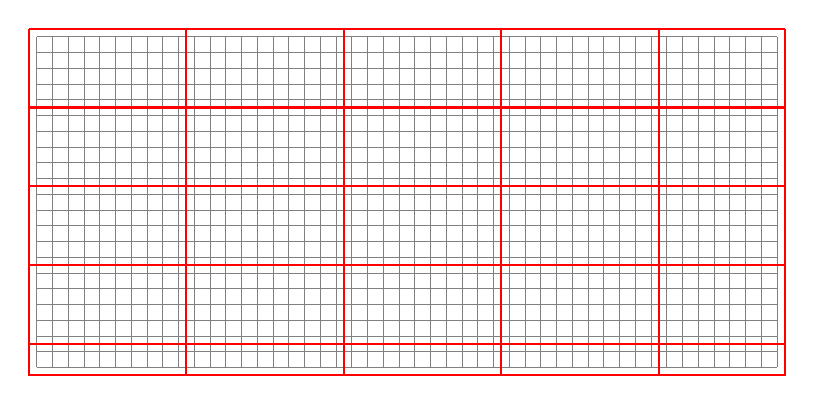
\begin{tikzpicture}
        % \foreach \x in {0,...,47}
        % \foreach \y in {-21,...,0}
        % {
        % \coordinate (ptc) at (\x, \y);
        % \fill ($ (0,0)!.2!(ptc) + (.1,-.1) $) circle (.75pt);
        % }
        
        \draw[xshift=.1cm, yshift=-.1cm, step=.2cm, gray, very thin] (0, 0) grid (9.4, -4.2);  %pts
        \draw[xstep=2cm, ystep=1cm, red, thick] (0, 0) grid (8, -4);  %proc center
        \draw[ystep=4mm, xstep=2cm, red, thick] (0,-4) grid (8,-4.41);
        \draw[ystep=1cm, xstep=1.6cm, red, thick] (8,0) grid (9.6,-4);
        \draw[red, thick] (8,-4) rectangle (9.6,-4.4);
      \end{tikzpicture}
    }
    \caption{Répartion d'une grille de taille $47$ par $21$ points sur $25$ processeurs.}
    \label{fig:rep_proc}
  \end{figure}
\end{frame}


\begin{frame}{Processeurs supplémentaires}
  \begin{blockitemize}{Existence inevitable}
  \item Souvent impossible d'utiliser tous les processeurs à disposition.
  \item Exemple : si $P$ est un nombre premier...
  \end{blockitemize}
  \begin{blockitemize}{Réutilisation}
  \item Le premier processeur non utilisé devient le processeur auxiliaire :
  \item Chargé de l'affichage
  \item Calcul la CFL
  \item Rassemble les erreurs $L^2$ locales et les somme
  \end{blockitemize}
  \begin{blockitemize}{Les autres...}
  \item sont perdus...
  \end{blockitemize}
\end{frame}

  
\subsection{Structure de la grille locale}

\begin{frame}{Une structure non triviale}
  \begin{blockitemize}{Intérêts}
  \item Accéder sans difficulté aux informations copiées depuis les processeurs voisins
  \item Avoir des contenants facilitant les communications entre processeurs
  \end{blockitemize}
  \begin{figure}
    \centering
    \hfill
    \resizebox{.45\textwidth}{!}{
      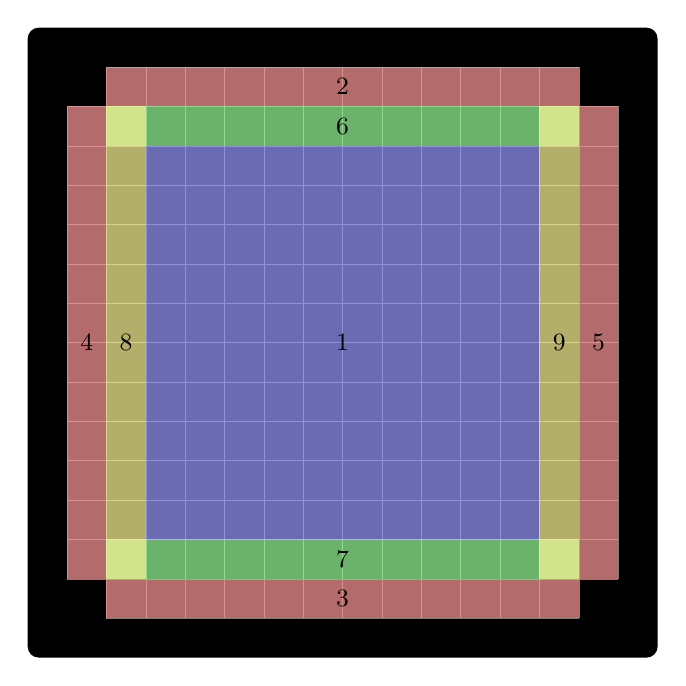
\begin{tikzpicture}
        \fill[black, rounded corners] (-4,4) rectangle (4,-4);
        \draw[step=0.5cm, gray, very thin] (-3, -3)    grid (3, 3);     %center
        \draw[step=0.5cm, gray, very thin] (-3, 3.5)   grid (3, 3);     %top
        \draw[step=0.5cm, gray, very thin] (-3, -3.5)  grid (3, -3);    %bottom
        \draw[step=0.5cm, gray, very thin] (-3.5, 3)   grid (-3, -3);   %left
        \draw[step=0.5cm, gray, very thin] (3, 3)      grid (3.5, -3);  %right

        \fill[blue!40!white, opacity=.7] (-2.5, -2.5) rectangle (2.5, 2.5);  %center
        \fill[red!40!white,  opacity=.7] (-3, 3.5)     rectangle (3, 3);      %top out   
        \fill[red!40!white,  opacity=.7] (-3, -3.5)    rectangle (3, -3);     %bottom out
        \fill[red!40!white,  opacity=.7] (-3.5, 3)     rectangle (-3, -3);    %left out 
        \fill[red!40!white,  opacity=.7] (3, 3)        rectangle (3.5, -3);   %right out

        \fill[green!40!white,  opacity=.7]  (-3, 3)    rectangle (3, 2.5);      %top in   
        \fill[green!40!white,  opacity=.7]  (-3, -2.5) rectangle (3, -3);     %bottom in
        \fill[yellow!40!white, opacity=.7] (-3, 3)    rectangle (-2.5, -3);    %left in 
        \fill[yellow!40!white, opacity=.7] (2.5, 3)   rectangle (3, -3);   %right in

        \node at (0,0)     () {\small 1}; %center
        \node at (0,3.25)  () {\small 2}; %top out
        \node at (0,-3.25) () {\small 3}; %bottom out
        \node at (-3.25,0) () {\small 4}; %left out
        \node at (3.25,0)  () {\small 5}; %right out
        \node at (0,2.75)  () {\small 6}; %top in
        \node at (0,-2.75) () {\small 7}; %bottom in
        \node at (-2.75,0) () {\small 8}; %left in
        \node at (2.75,0)  () {\small 9}; %right in
      \end{tikzpicture}
    }
    \hfill
    \begin{minipage}[b]{.3\textwidth}
      \begin{enumerate}
      \item \texttt{center}
      \item \texttt{top\_out}
      \item \texttt{bottom\_out}
      \item \texttt{left\_out}
      \item \texttt{right\_out}
      \item \texttt{top\_in}
      \item \texttt{bottom\_in}
      \item \texttt{left\_in}
      \item \texttt{right\_in}
      \end{enumerate}
    \end{minipage}
    \hfill
\end{figure}
\end{frame}

\begin{frame}{Communication entre grilles étendues}{Exemple de communication}
  \centering
  \begin{minipage}{.5\textwidth}
    \resizebox{\textwidth}{!}{
      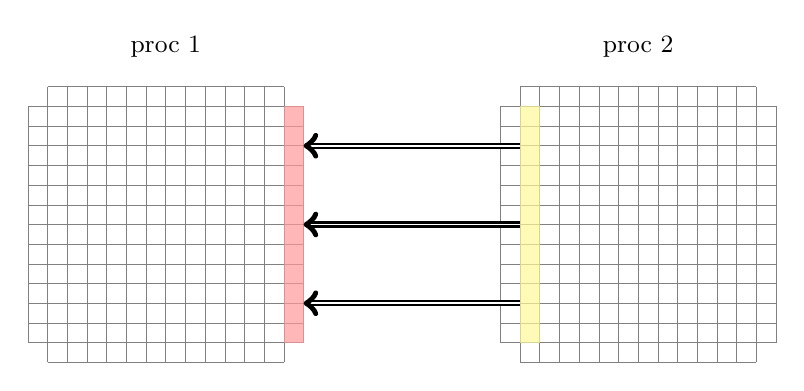
\begin{tikzpicture}
        % \fill[black, rounded corners] (-2.5, 3) rectangle (7,-3);
        \coordinate (lt) at (-1.5,1.5);
        \coordinate (rt) at (1.5,1.5);
        \coordinate (lb) at (-1.5,-1.5);
        \coordinate (rb) at (1.5,-1.5);
        
        \coordinate (ult) at (-1.5,1.75);
        \coordinate (llt) at (-1.75,1.5);
        \coordinate (rrb) at (1.75,-1.5);
        \coordinate (brb) at (1.5,-1.75);

        \coordinate (lrt) at (1.5,1.25);
        \coordinate (brt) at (1.5,1.25);
        \coordinate (tlb) at (-1.5,-1.25);
        \coordinate (rlb) at (-1.25,-1.5);

        \coordinate (shift) at (5.9999,0);

        \node at ($ (lt)!.5!(rt) + (0,.75)$) () {\small proc 1};
        \node at ($ (lt)!.5!(rt) + (0,.75) + (shift) $) () {\small proc 2};

        \draw[step=0.25cm, gray, very thin] (lt)    grid (rb);   %center
        \draw[step=0.25cm, gray, very thin] (ult)   grid (rt);   %top
        \draw[step=0.25cm, gray, very thin] (lb)    grid (brb);  %bottom
        \draw[step=0.25cm, gray, very thin] (llt)   grid (lb);   %left
        \draw[step=0.25cm, gray, very thin] (rt)    grid (rrb);  %right

        \draw[step=0.25cm, gray, very thin] ($ (lt) + (shift)  $)  grid ($ (rb) + (shift)  $);   %center
        \draw[step=0.25cm, gray, very thin] ($ (ult) + (shift) $)  grid ($ (rt) + (shift)  $);   %top
        \draw[step=0.25cm, gray, very thin] ($ (lb) + (shift)  $)  grid ($ (brb) + (shift) $);   %bottom
        \draw[step=0.25cm, gray, very thin] ($ (llt) + (shift) $)  grid ($ (lb) + (shift)  $);   %left
        \draw[step=0.25cm, gray, very thin] ($ (rt) + (shift)  $)  grid ($ (rrb) + (shift) $);   %right

        \fill[red!40!white,  opacity=.7]   (rt) rectangle (rrb);   %left out 
        \fill[yellow!40!white,  opacity=.7] ($ (lt) + (shift) $) rectangle ($ (rlb) + (shift) $);  %left in
        \draw[<-, thick, double] ($ ($(rt)!.5!(rrb)$) + (0.125,0) $) to ($ ($ ($(lt)!.5!(rlb)$) + (shift) $) + (-.125, 0) $);
        \draw[<-, thick, double] ($ ($(rt)!.5!(rrb)$) + (0.125, 1) $) to ($ ($ ($(lt)!.5!(rlb)$) + (shift) $) + (-.125, 1) $);
        \draw[<-, thick, double] ($ ($(rt)!.5!(rrb)$) + (0.125, -1) $) to ($ ($ ($(lt)!.5!(rlb)$) + (shift) $) + (-.125, -1) $);
      \end{tikzpicture}
    }
  \end{minipage}
  \hspace{50pt}
  \begin{minipage}[t]{.3\textwidth}
    \small
    Communication droite vers gauche : copie \texttt{right\_in} de proc 1 dans \texttt{left\_out} de proc 2.
  \end{minipage}

  \vspace{50pt}
  \begin{minipage}{.5\textwidth}
  \resizebox{\textwidth}{!}{
    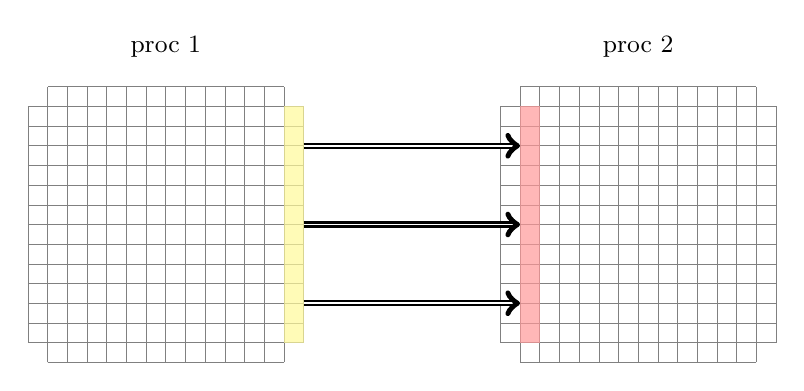
\begin{tikzpicture}
      % \fill[black, rounded corners] (-2.5, 3) rectangle (7,-3);
      \coordinate (lt) at (-1.5,1.5);
      \coordinate (rt) at (1.5,1.5);
      \coordinate (lb) at (-1.5,-1.5);
      \coordinate (rb) at (1.5,-1.5);
      
      \coordinate (ult) at (-1.5,1.75);
      \coordinate (llt) at (-1.75,1.5);
      \coordinate (rrb) at (1.75,-1.5);
      \coordinate (brb) at (1.5,-1.75);

      \coordinate (lrt) at (1.5,1.25);
      \coordinate (brt) at (1.5,1.25);
      \coordinate (tlb) at (-1.5,-1.25);
      \coordinate (rlb) at (-1.25,-1.5);

      \coordinate (shift) at (5.9999,0);

      \node at ($ (lt)!.5!(rt) + (0,.75)$) () {\small proc 1};
      \node at ($ (lt)!.5!(rt) + (0,.75) + (shift) $) () {\small proc 2};

      \draw[step=0.25cm, gray, very thin] (lt)    grid (rb);   %center
      \draw[step=0.25cm, gray, very thin] (ult)   grid (rt);   %top
      \draw[step=0.25cm, gray, very thin] (lb)    grid (brb);  %bottom
      \draw[step=0.25cm, gray, very thin] (llt)   grid (lb);   %left
      \draw[step=0.25cm, gray, very thin] (rt)    grid (rrb);  %right

      \draw[step=0.25cm, gray, very thin] ($ (lt) + (shift)  $)  grid ($ (rb) + (shift)  $);   %center
      \draw[step=0.25cm, gray, very thin] ($ (ult) + (shift) $)  grid ($ (rt) + (shift)  $);   %top
      \draw[step=0.25cm, gray, very thin] ($ (lb) + (shift)  $)  grid ($ (brb) + (shift) $);   %bottom
      \draw[step=0.25cm, gray, very thin] ($ (llt) + (shift) $)  grid ($ (lb) + (shift)  $);   %left
      \draw[step=0.25cm, gray, very thin] ($ (rt) + (shift)  $)  grid ($ (rrb) + (shift) $);   %right

      \fill[yellow!40!white,  opacity=.7]   (rt) rectangle (rrb);   %left out 
      \fill[red!40!white,  opacity=.7] ($ (lt) + (shift) $) rectangle ($ (rlb) + (shift) $);  %left in
      \draw[->, thick, double] ($ ($(rt)!.5!(rrb)$) + (0.125,0) $)   to ($ ($ ($(lt)!.5!(rlb)$) + (shift) $) + (-.125, 0) $);
      \draw[->, thick, double] ($ ($(rt)!.5!(rrb)$) + (0.125, 1) $)  to ($ ($ ($(lt)!.5!(rlb)$) + (shift) $) + (-.125, 1) $);
      \draw[->, thick, double] ($ ($(rt)!.5!(rrb)$) + (0.125, -1) $) to ($ ($ ($(lt)!.5!(rlb)$) + (shift) $) + (-.125, -1) $);
    \end{tikzpicture}
  }
  \end{minipage}
  \hspace{50pt}
  \begin{minipage}[t]{.3\textwidth}
    \small
    Communication gauche vers droite : copie \texttt{right\_out} de proc 1 dans \texttt{left\_in} de proc 2.
  \end{minipage}
\end{frame}

\end{document}
%%% Local Variables:
%%% mode: latex
%%% TeX-master: t
%%% End:
